\documentclass[12pt]{article}

\usepackage{geometry}
\geometry{margin=1in}

\usepackage{graphicx}
\usepackage{booktabs}
\usepackage{amsmath}
\usepackage{amssymb}
\usepackage{natbib}
\usepackage{setspace}
\usepackage{hyperref}

\onehalfspacing

\title{Supplementary Materials: \\
Organisms Write Evolution Through Epigenomic Inheritance}

\author{}
\date{}

\begin{document}

\maketitle

\section*{Supplementary Figures and Analyses}

This document provides supplementary figures and detailed analyses supporting the main manuscript. The following seven figures present additional perspectives on algorithm performance, convergence dynamics, and component-wise learning across all experimental conditions.

\newpage

\section*{Supplementary Figure S1: Compositional Advantage Ratios}

\begin{figure}[h!]
\centering
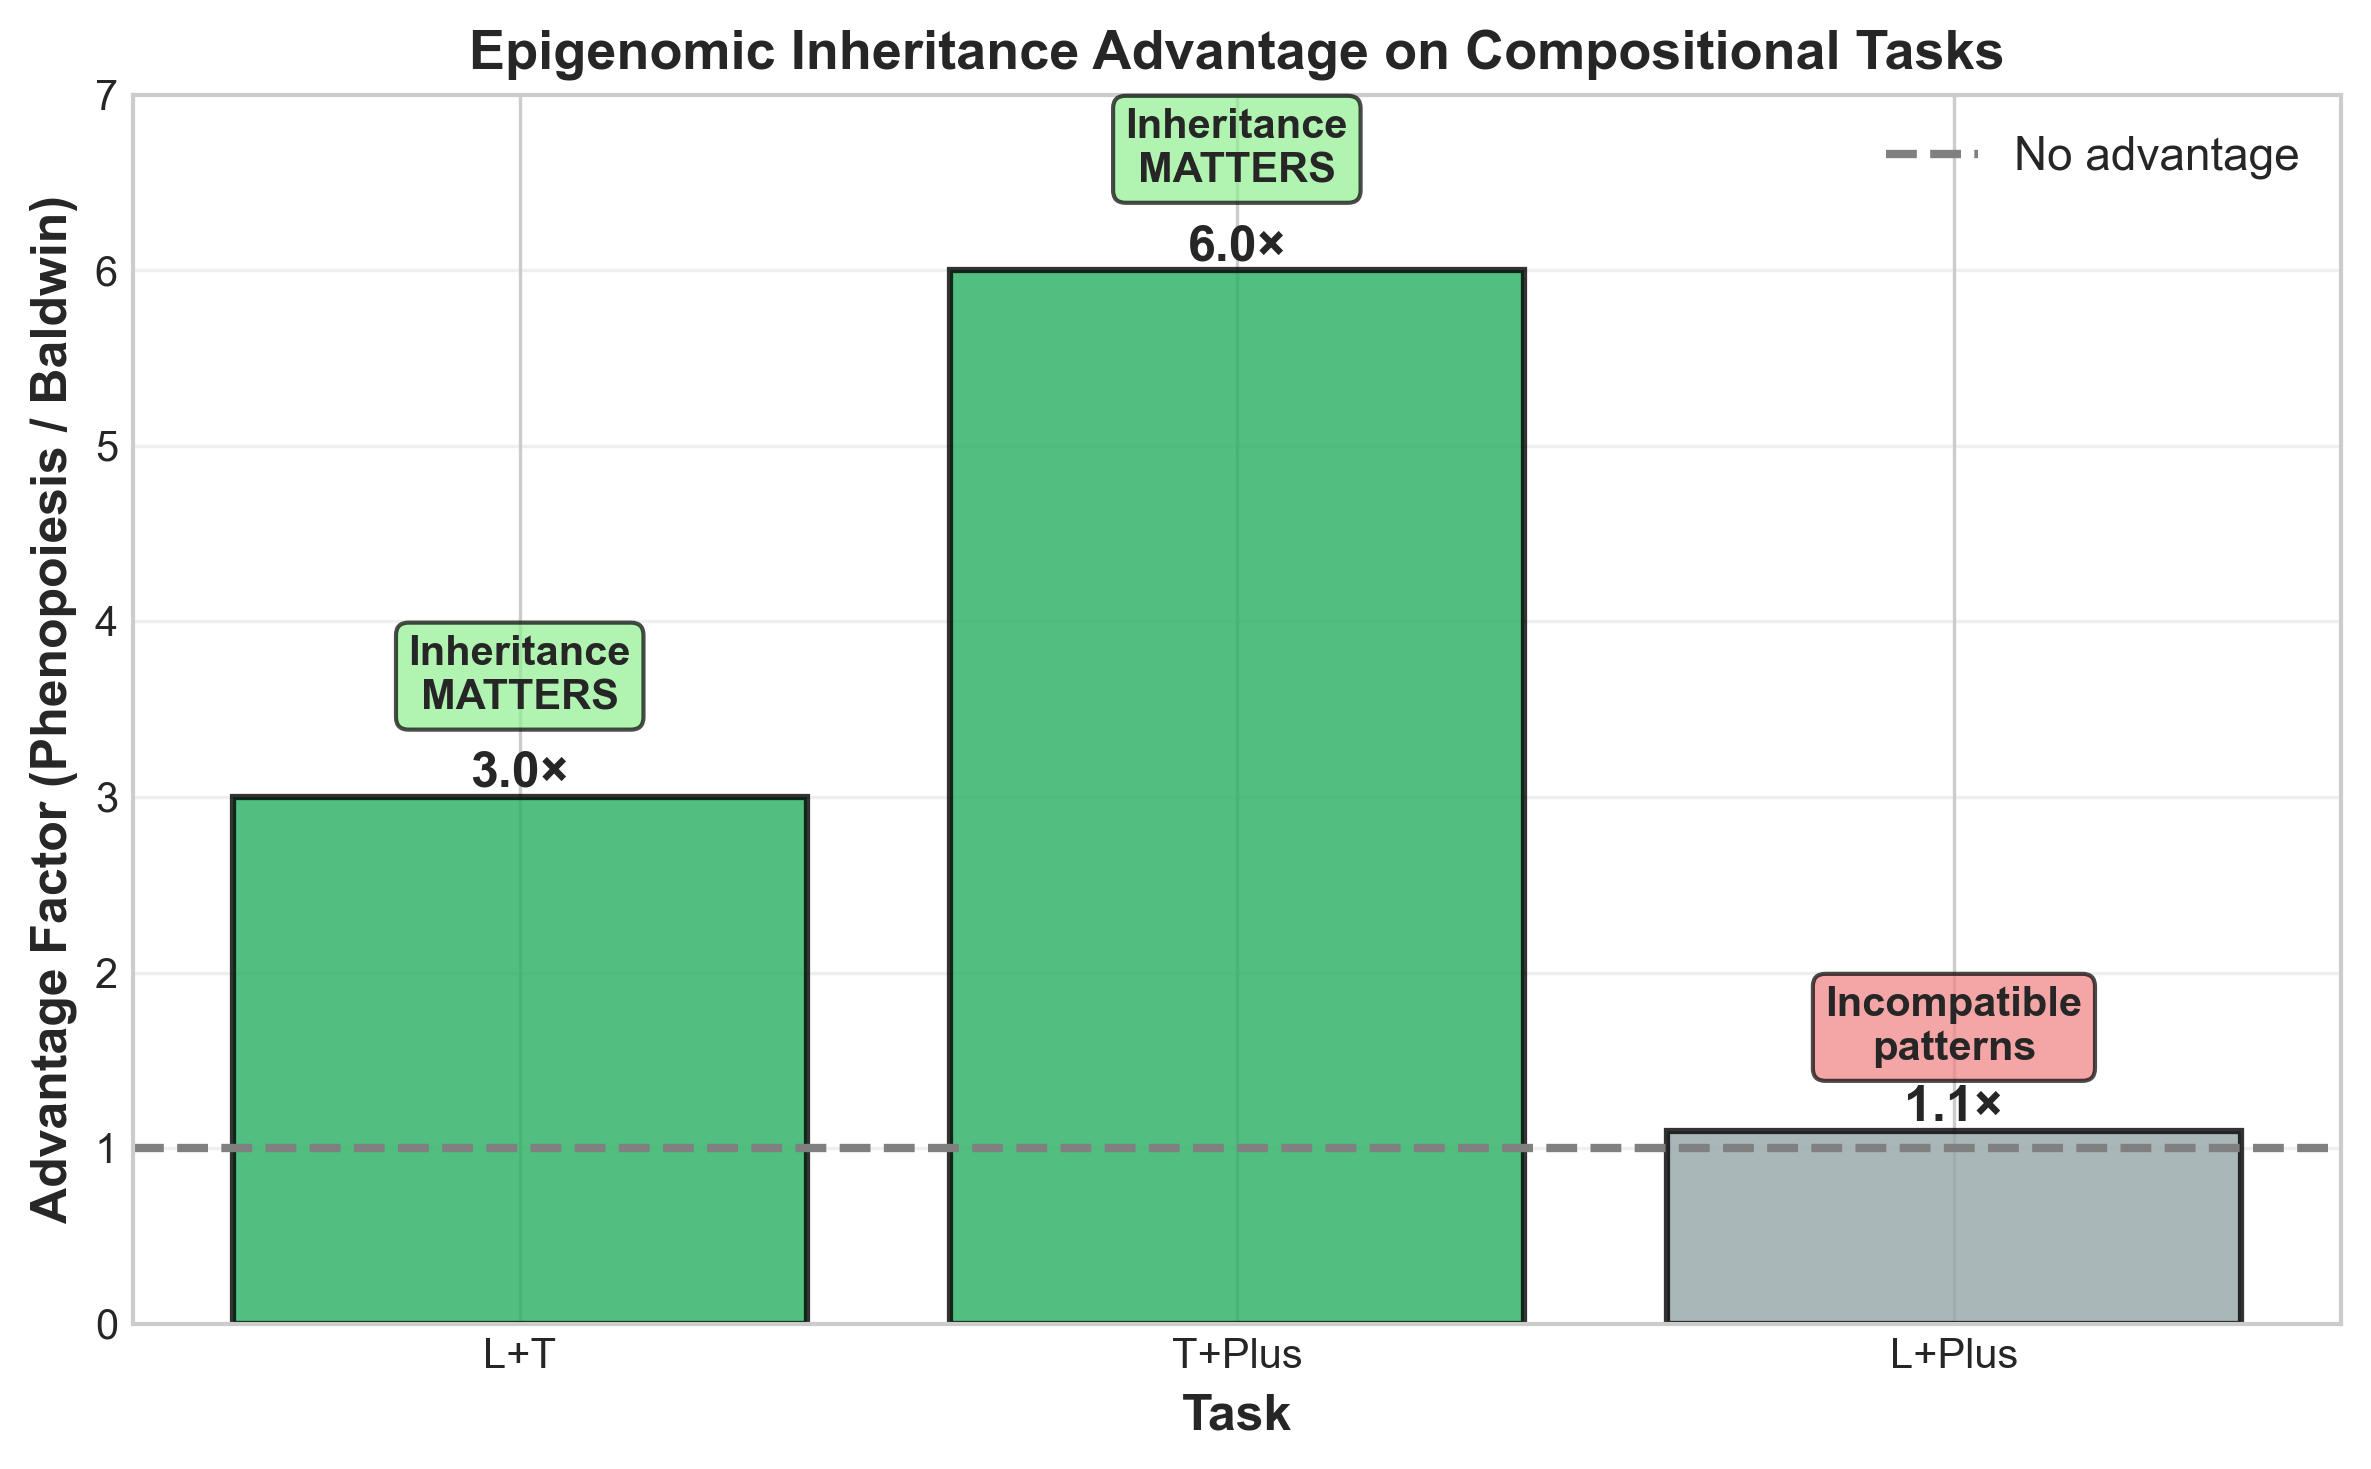
\includegraphics[width=6.5in]{compositional_advantage_ratios.png}
\caption{\textbf{Phenopoiesis Advantage Factors Across Compositional Tasks.}
Bar plot showing the fitness advantage ratio of Phenopoiesis compared to Baldwin Effect for each compositional task. Advantage calculated as: Fitness(Phenopoiesis) / Fitness(Baldwin).
\textbf{Key findings:} L+T task shows 3.0$\times$ advantage, indicating that epigenomic inheritance of learned L pattern enables efficient T pattern learning in offspring. T+Plus task shows 6.0$\times$ advantage, reflecting greater difficulty of learning Plus pattern sequentially after T. L+Plus task shows 1.1$\times$ no advantage, demonstrating that geometric pattern incompatibility prevents inheritance benefit. This demonstrates that extended agency provides advantage only when problem structure permits sequential, independent learning of components.}
\label{SFig:1}
\end{figure}

\newpage

\section*{Supplementary Figure S2: Component-Wise Fitness Analysis}

\begin{figure}[h!]
\centering
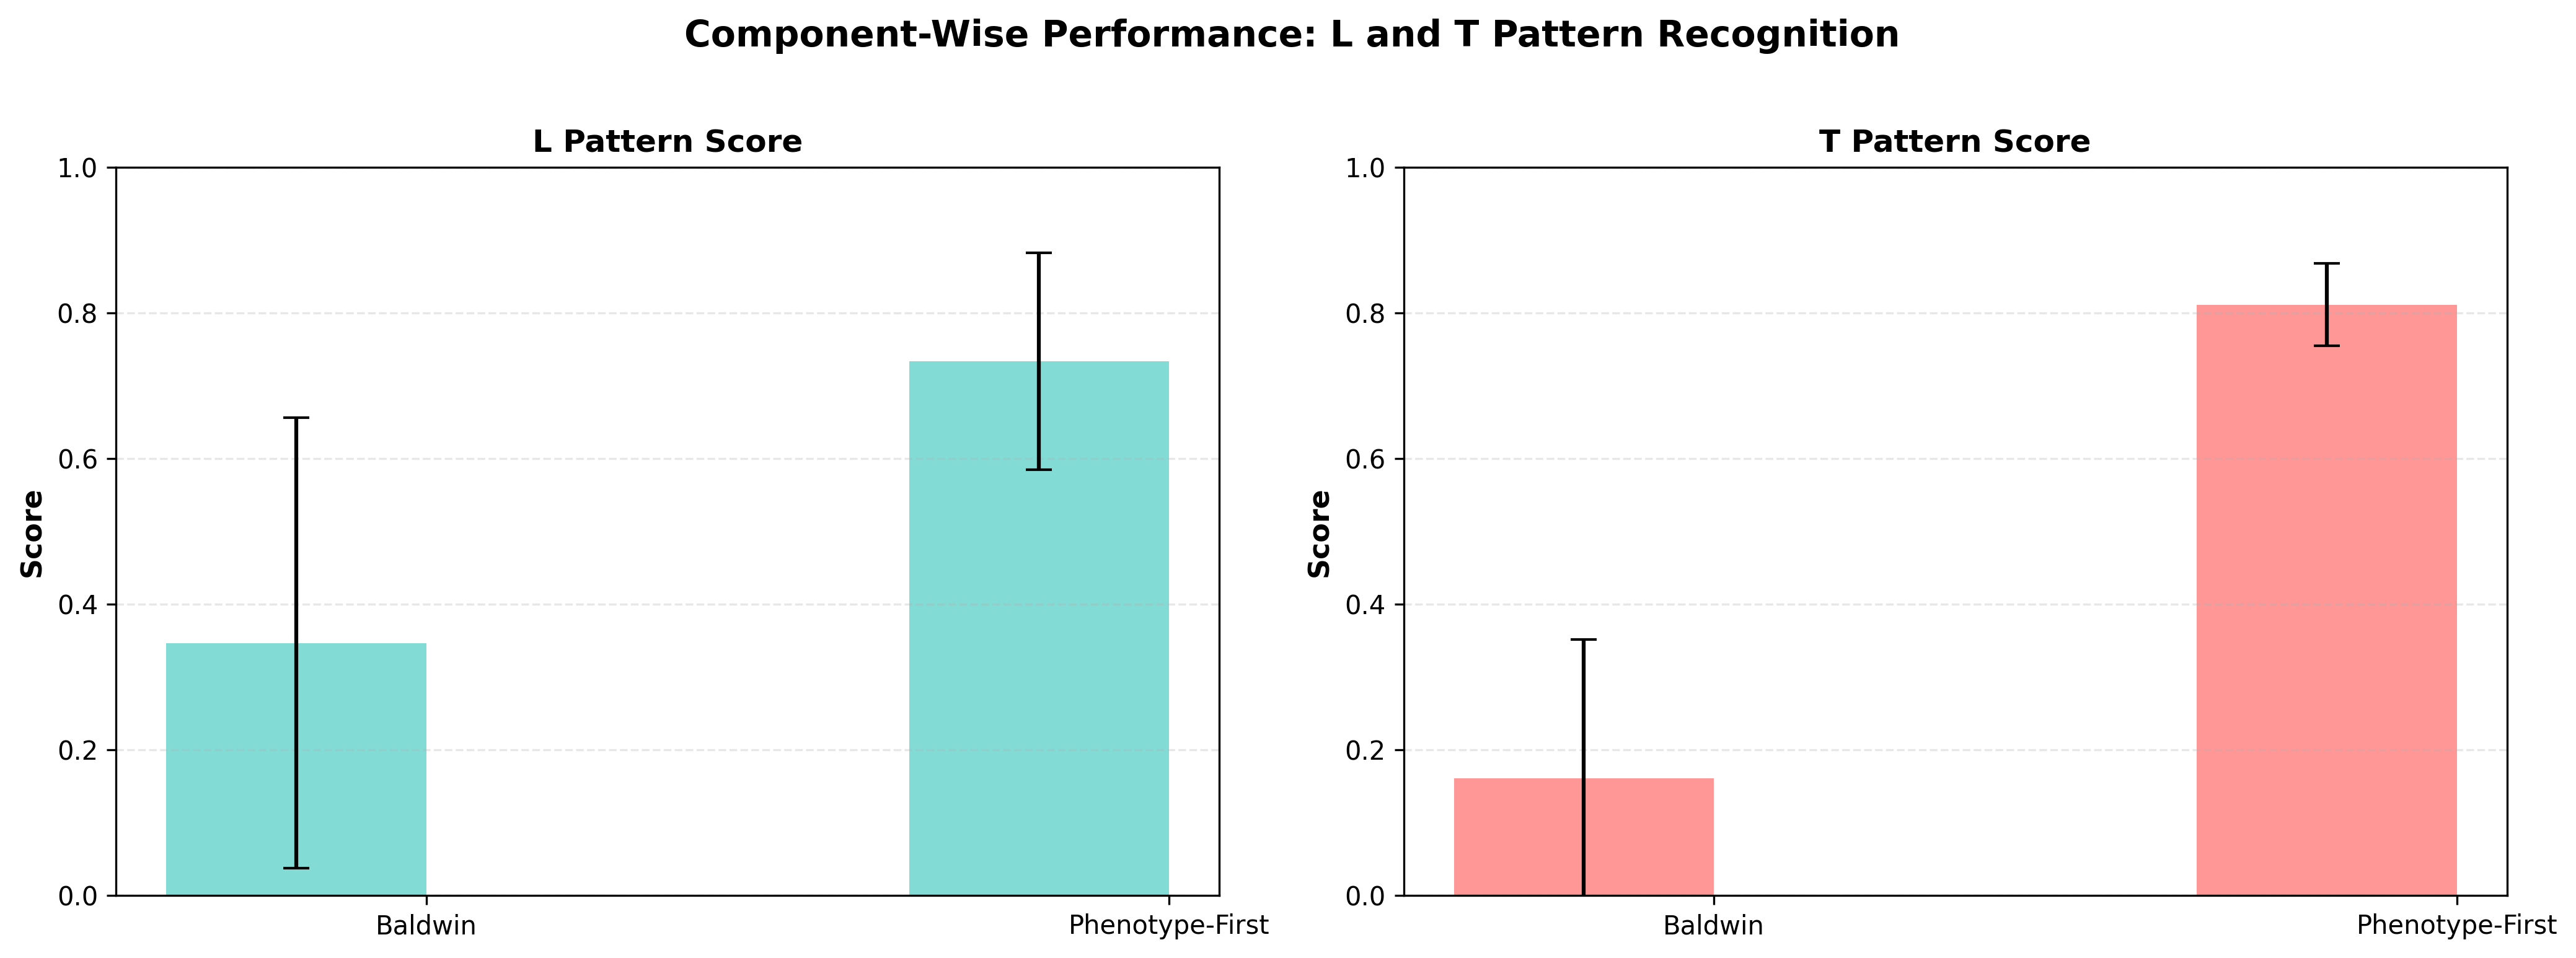
\includegraphics[width=6.5in]{compositional_component_scores.png}
\caption{\textbf{Component Fitness Scores for Compositional Tasks.}
Separate fitness evaluations for L, T, and Plus components on compositional tasks. For each task, component fitness = (cells matched for that component) / (total cells defining that component).
\textbf{Key findings:} Phenopoiesis maintains high component-specific fitness for both components on learnable tasks (L+T and T+Plus), indicating that inheritance enables organisms to preserve learned components while learning new ones. Baldwin Effect shows lower and more variable component fitness, reflecting inability to accumulate knowledge. L+Plus shows low component fitness for both algorithms equally, confirming that geometric interference, not learning mechanism, limits performance.}
\label{SFig:2}
\end{figure}

\newpage

\section*{Supplementary Figure S3: Convergence Time Analysis}

\begin{figure}[h!]
\centering
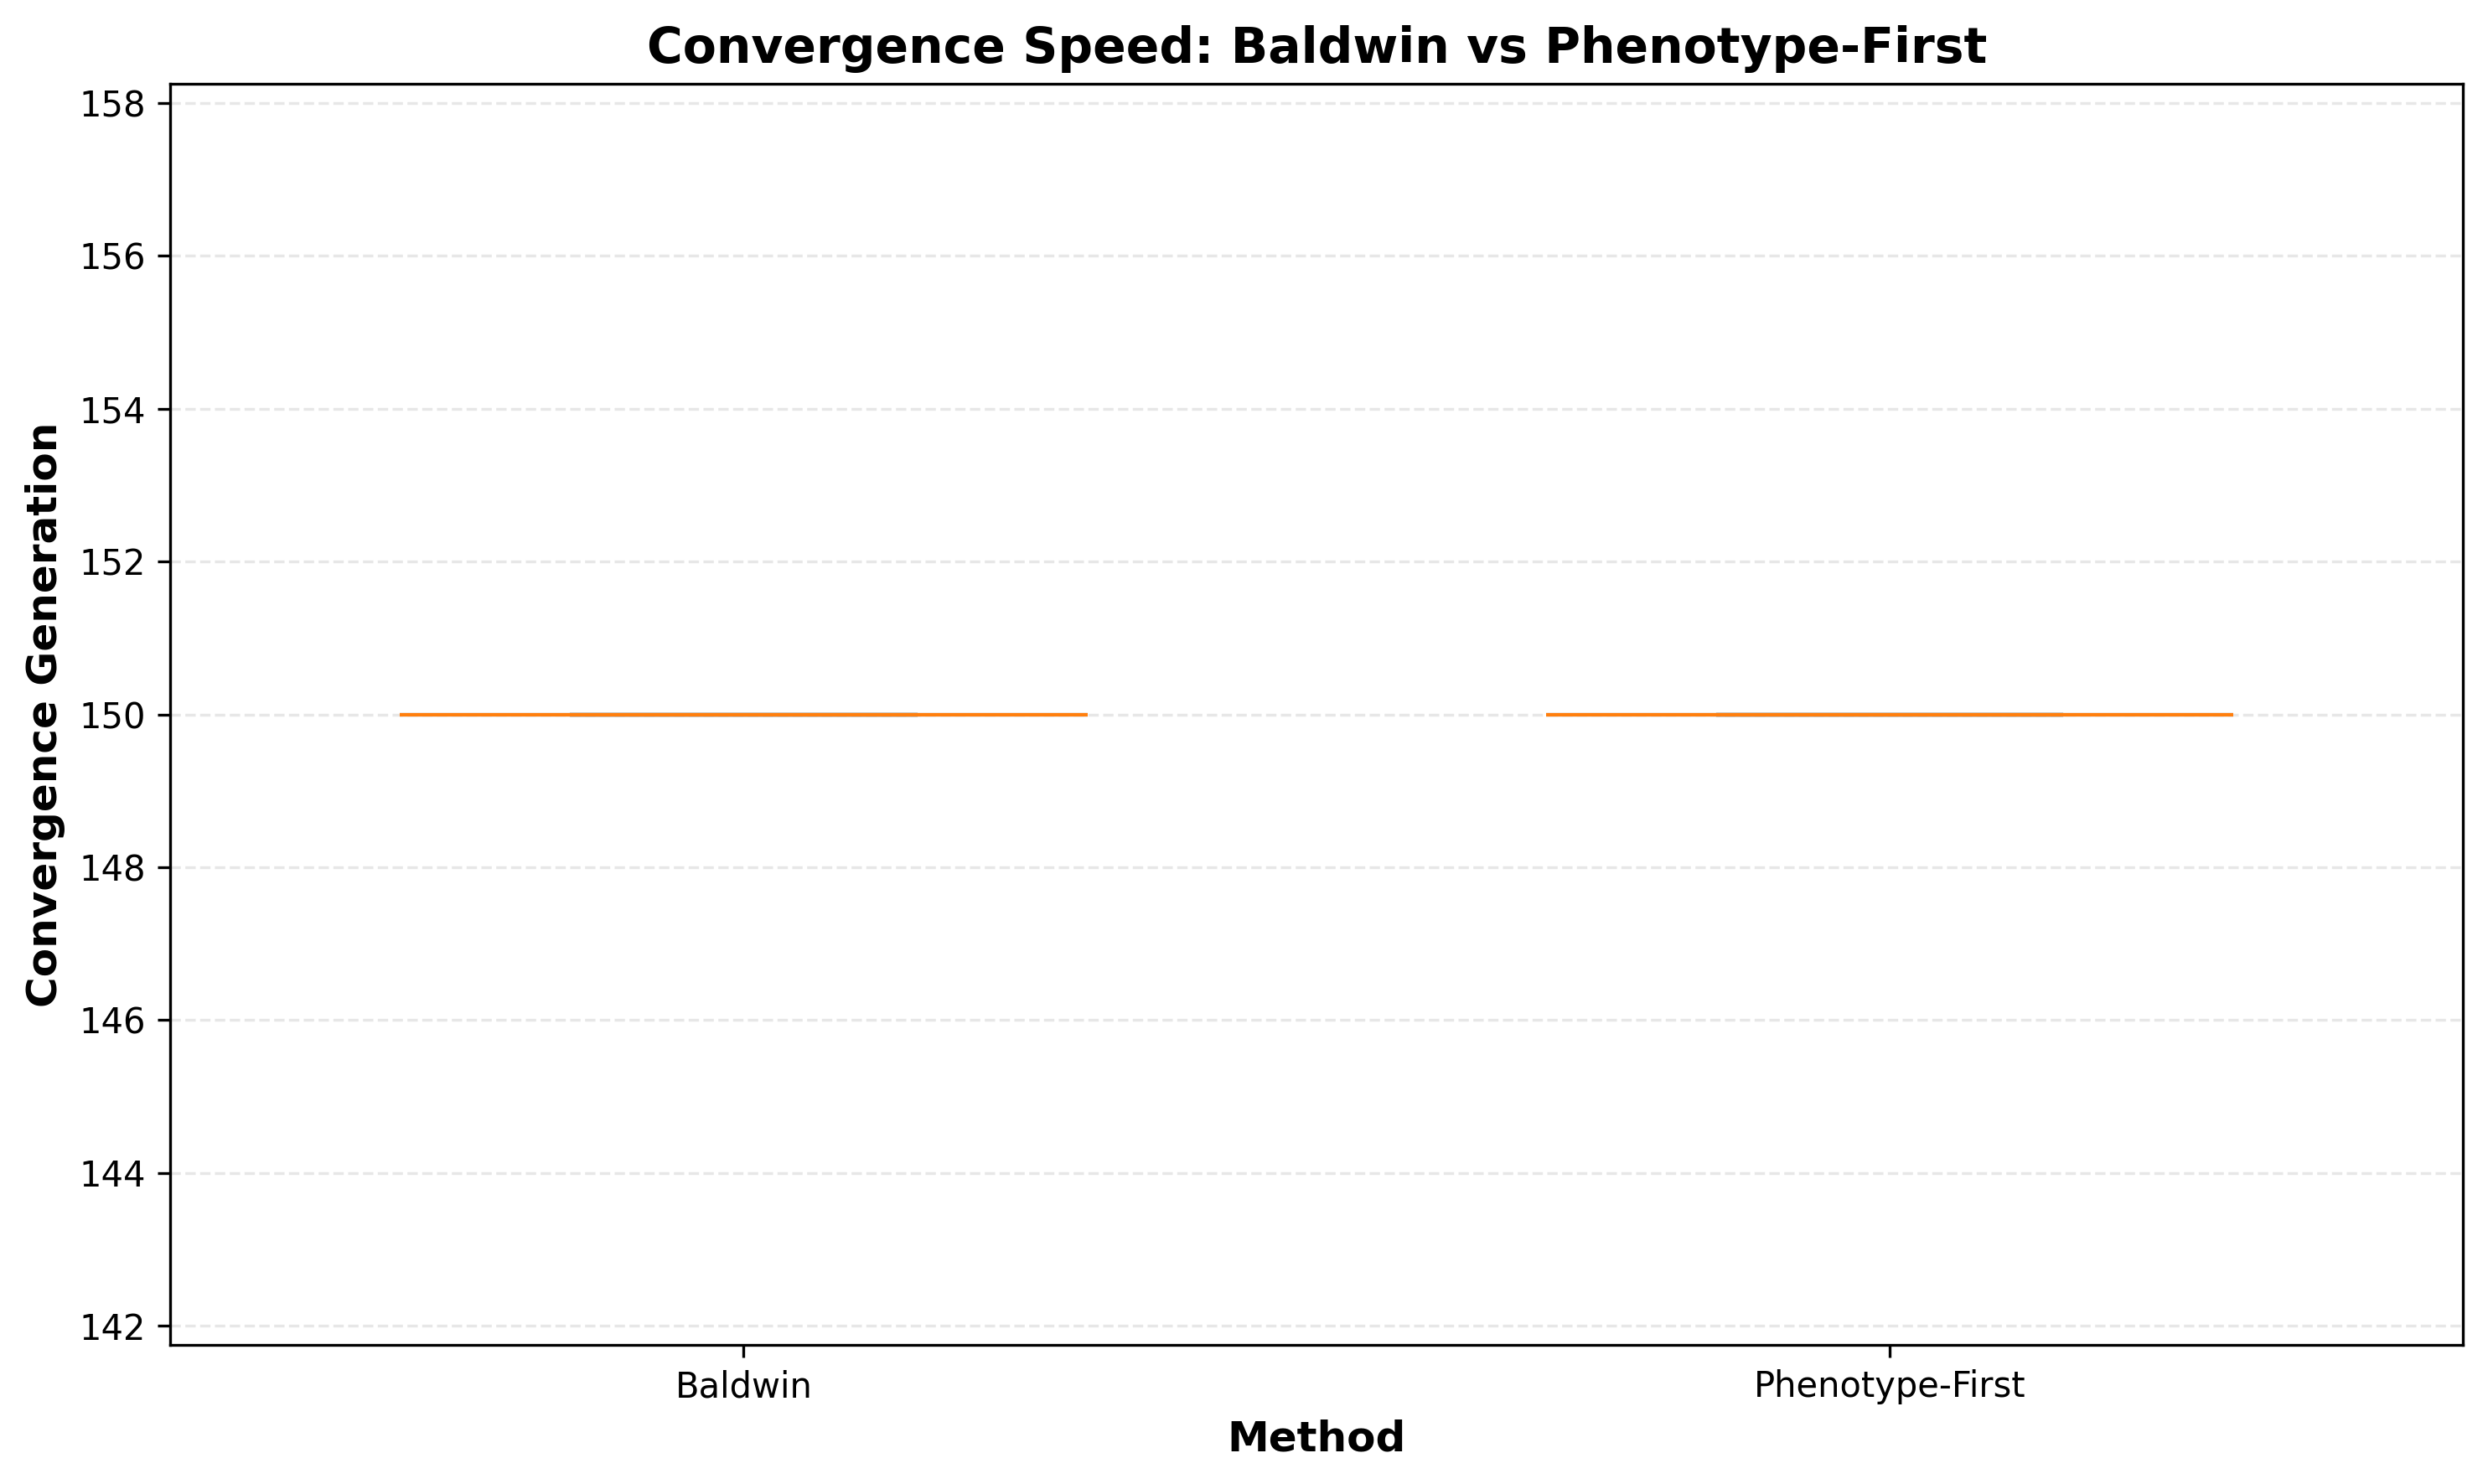
\includegraphics[width=6.5in]{compositional_convergence.png}
\caption{\textbf{Convergence Speed: Generation to 80\% Final Fitness.}
Box plots showing the distribution of convergence times (generation at which mean fitness first reaches 80\% of final value) across 30 runs for each algorithm-task combination.
\textbf{Key findings:} Gene-Centric GA shows slow or no convergence on compositional tasks. Phenopoiesis converges dramatically faster on learnable tasks (L+T and T+Plus) with median convergence in early generations (20-40 generations), reflecting that inheritance of learned patterns accelerates subsequent learning. L+Plus shows no convergence advantage for either mechanism, as both plateau at low fitness.}
\label{SFig:3}
\end{figure}

\newpage

\section*{Supplementary Figure S4: Fitness Variance Analysis}

\begin{figure}[h!]
\centering
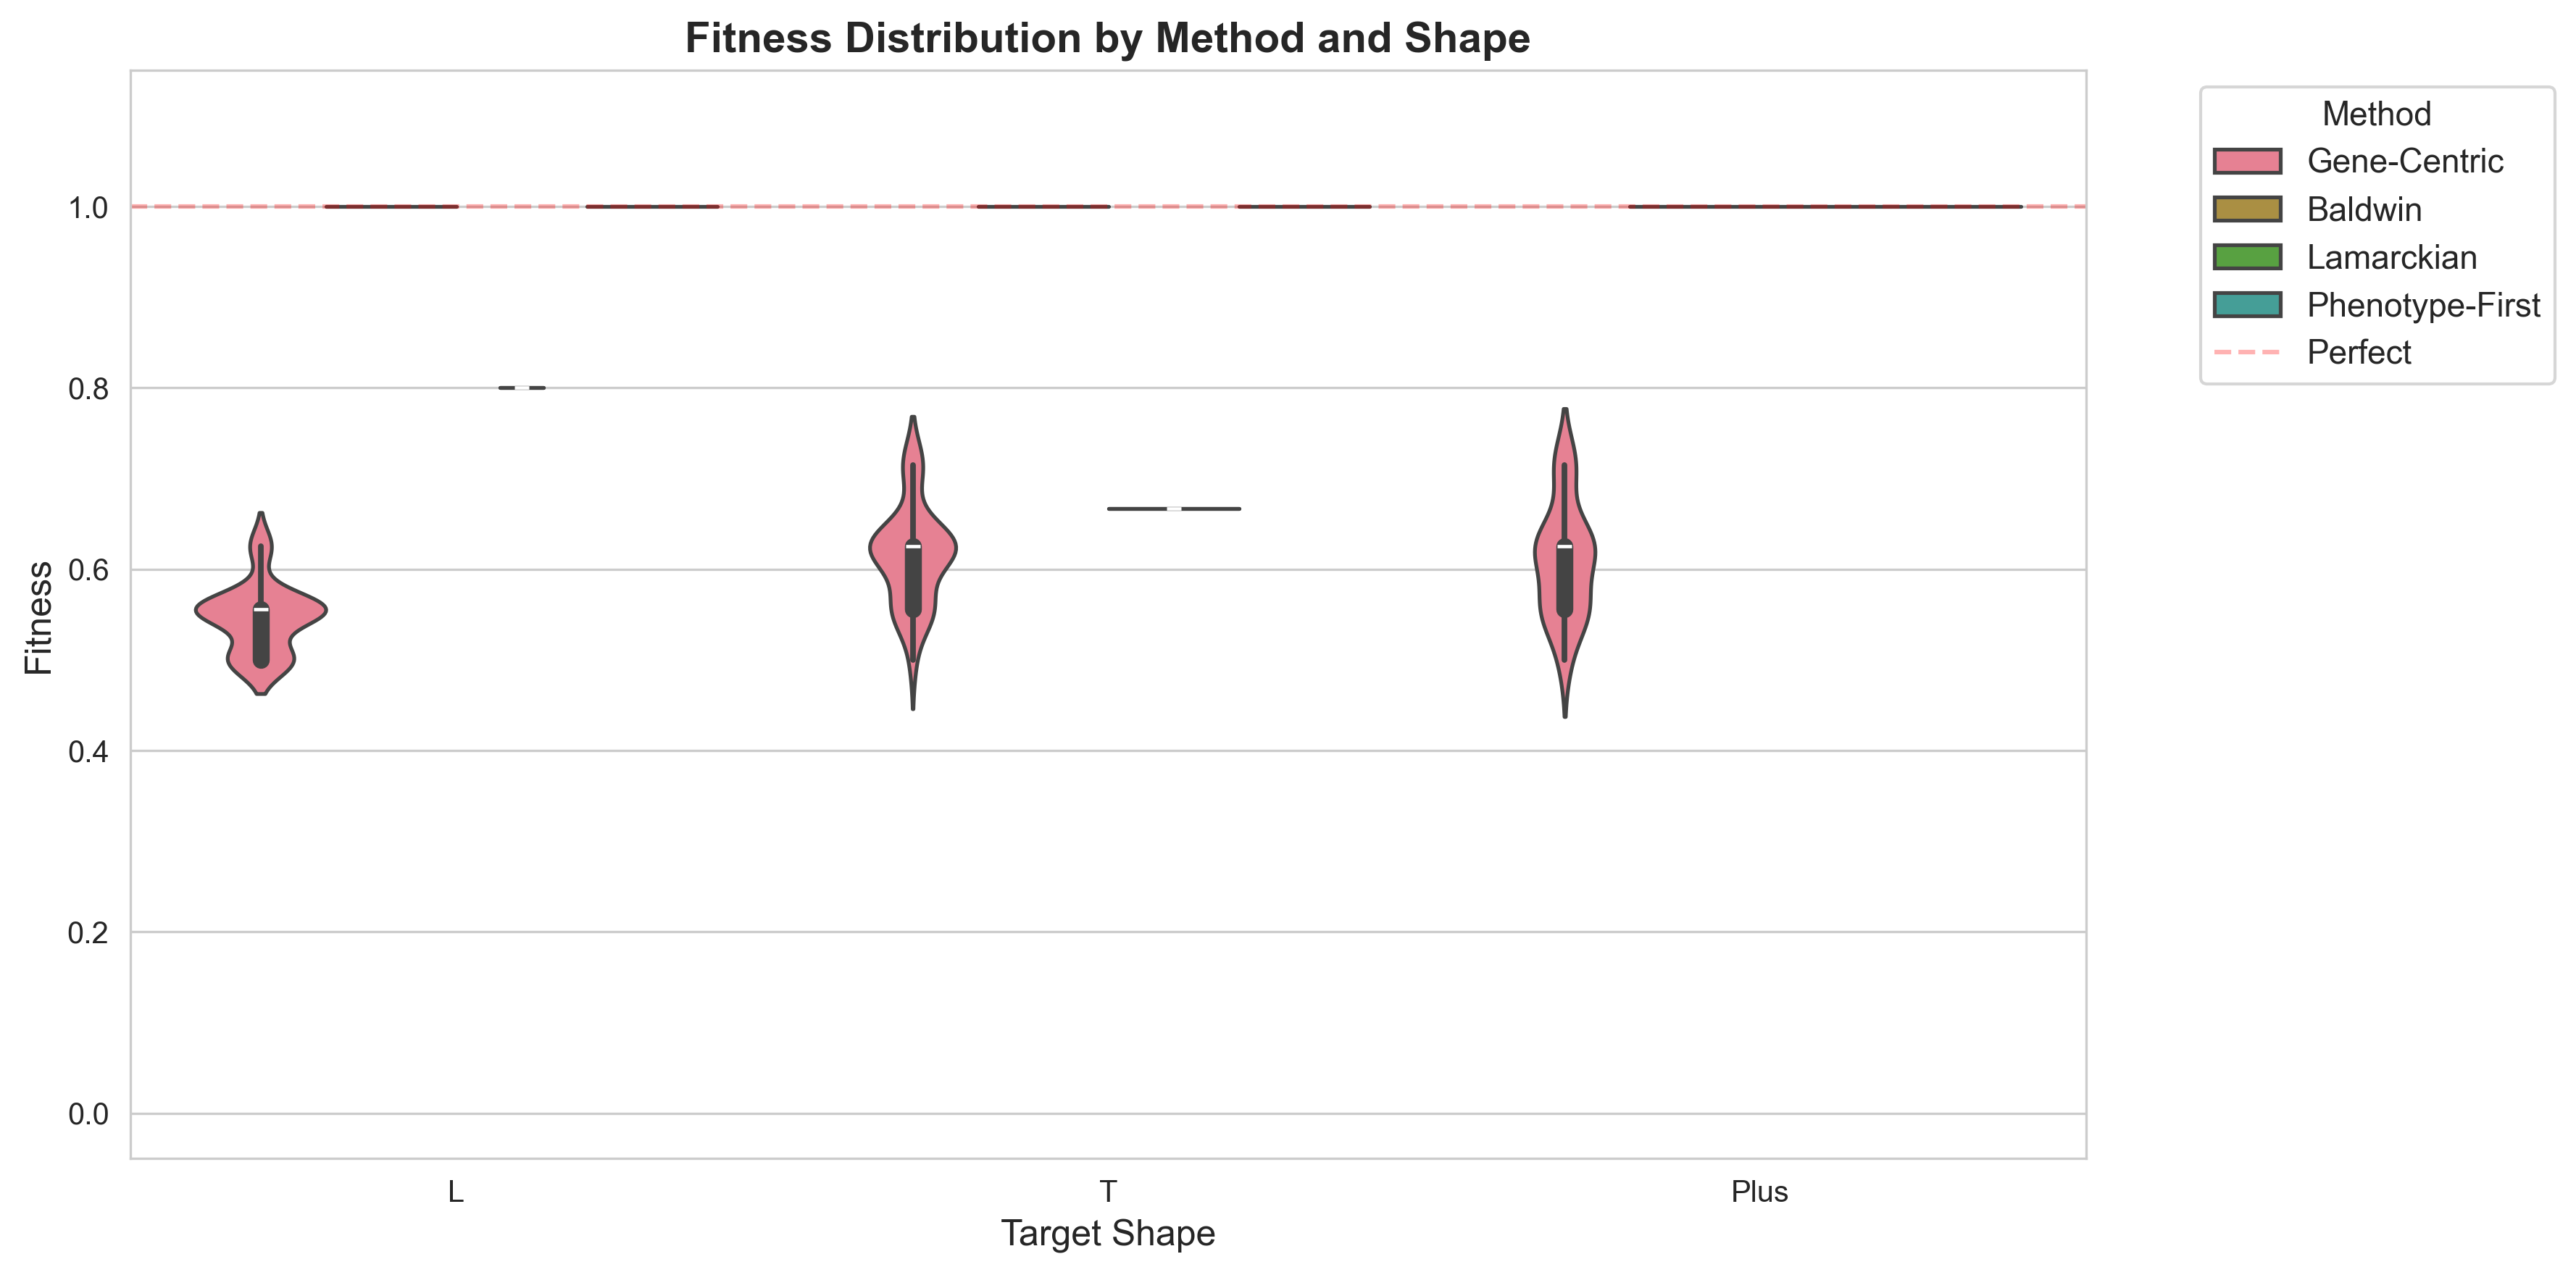
\includegraphics[width=6.5in]{plot_violin_fitness.png}
\caption{\textbf{Fitness Distribution Variance: Violin Plots Across Conditions.}
Violin plots showing the probability density distribution of fitness values across 30 independent runs for each algorithm-task combination. Violin width indicates distribution density at each fitness level.
\textbf{Key findings:} Gene-Centric GA shows broad, variable distributions on all tasks, reflecting random search. Baldwin Effect shows broad distributions on compositional tasks (s.d. = 0.123 on T+Plus), indicating stochastic learning. Phenopoiesis shows tight, narrow distributions on learnable compositional tasks, with perfectly sharp peak on T+Plus (s.d. = 0.0, all 30 runs identical), indicating deterministic convergence to a single reliable solution. L+Plus shows similarly broad distributions for both algorithms.}
\label{SFig:4}
\end{figure}

\newpage

\section*{Supplementary Figure S5: Pattern Interference Analysis}

\begin{figure}[h!]
\centering
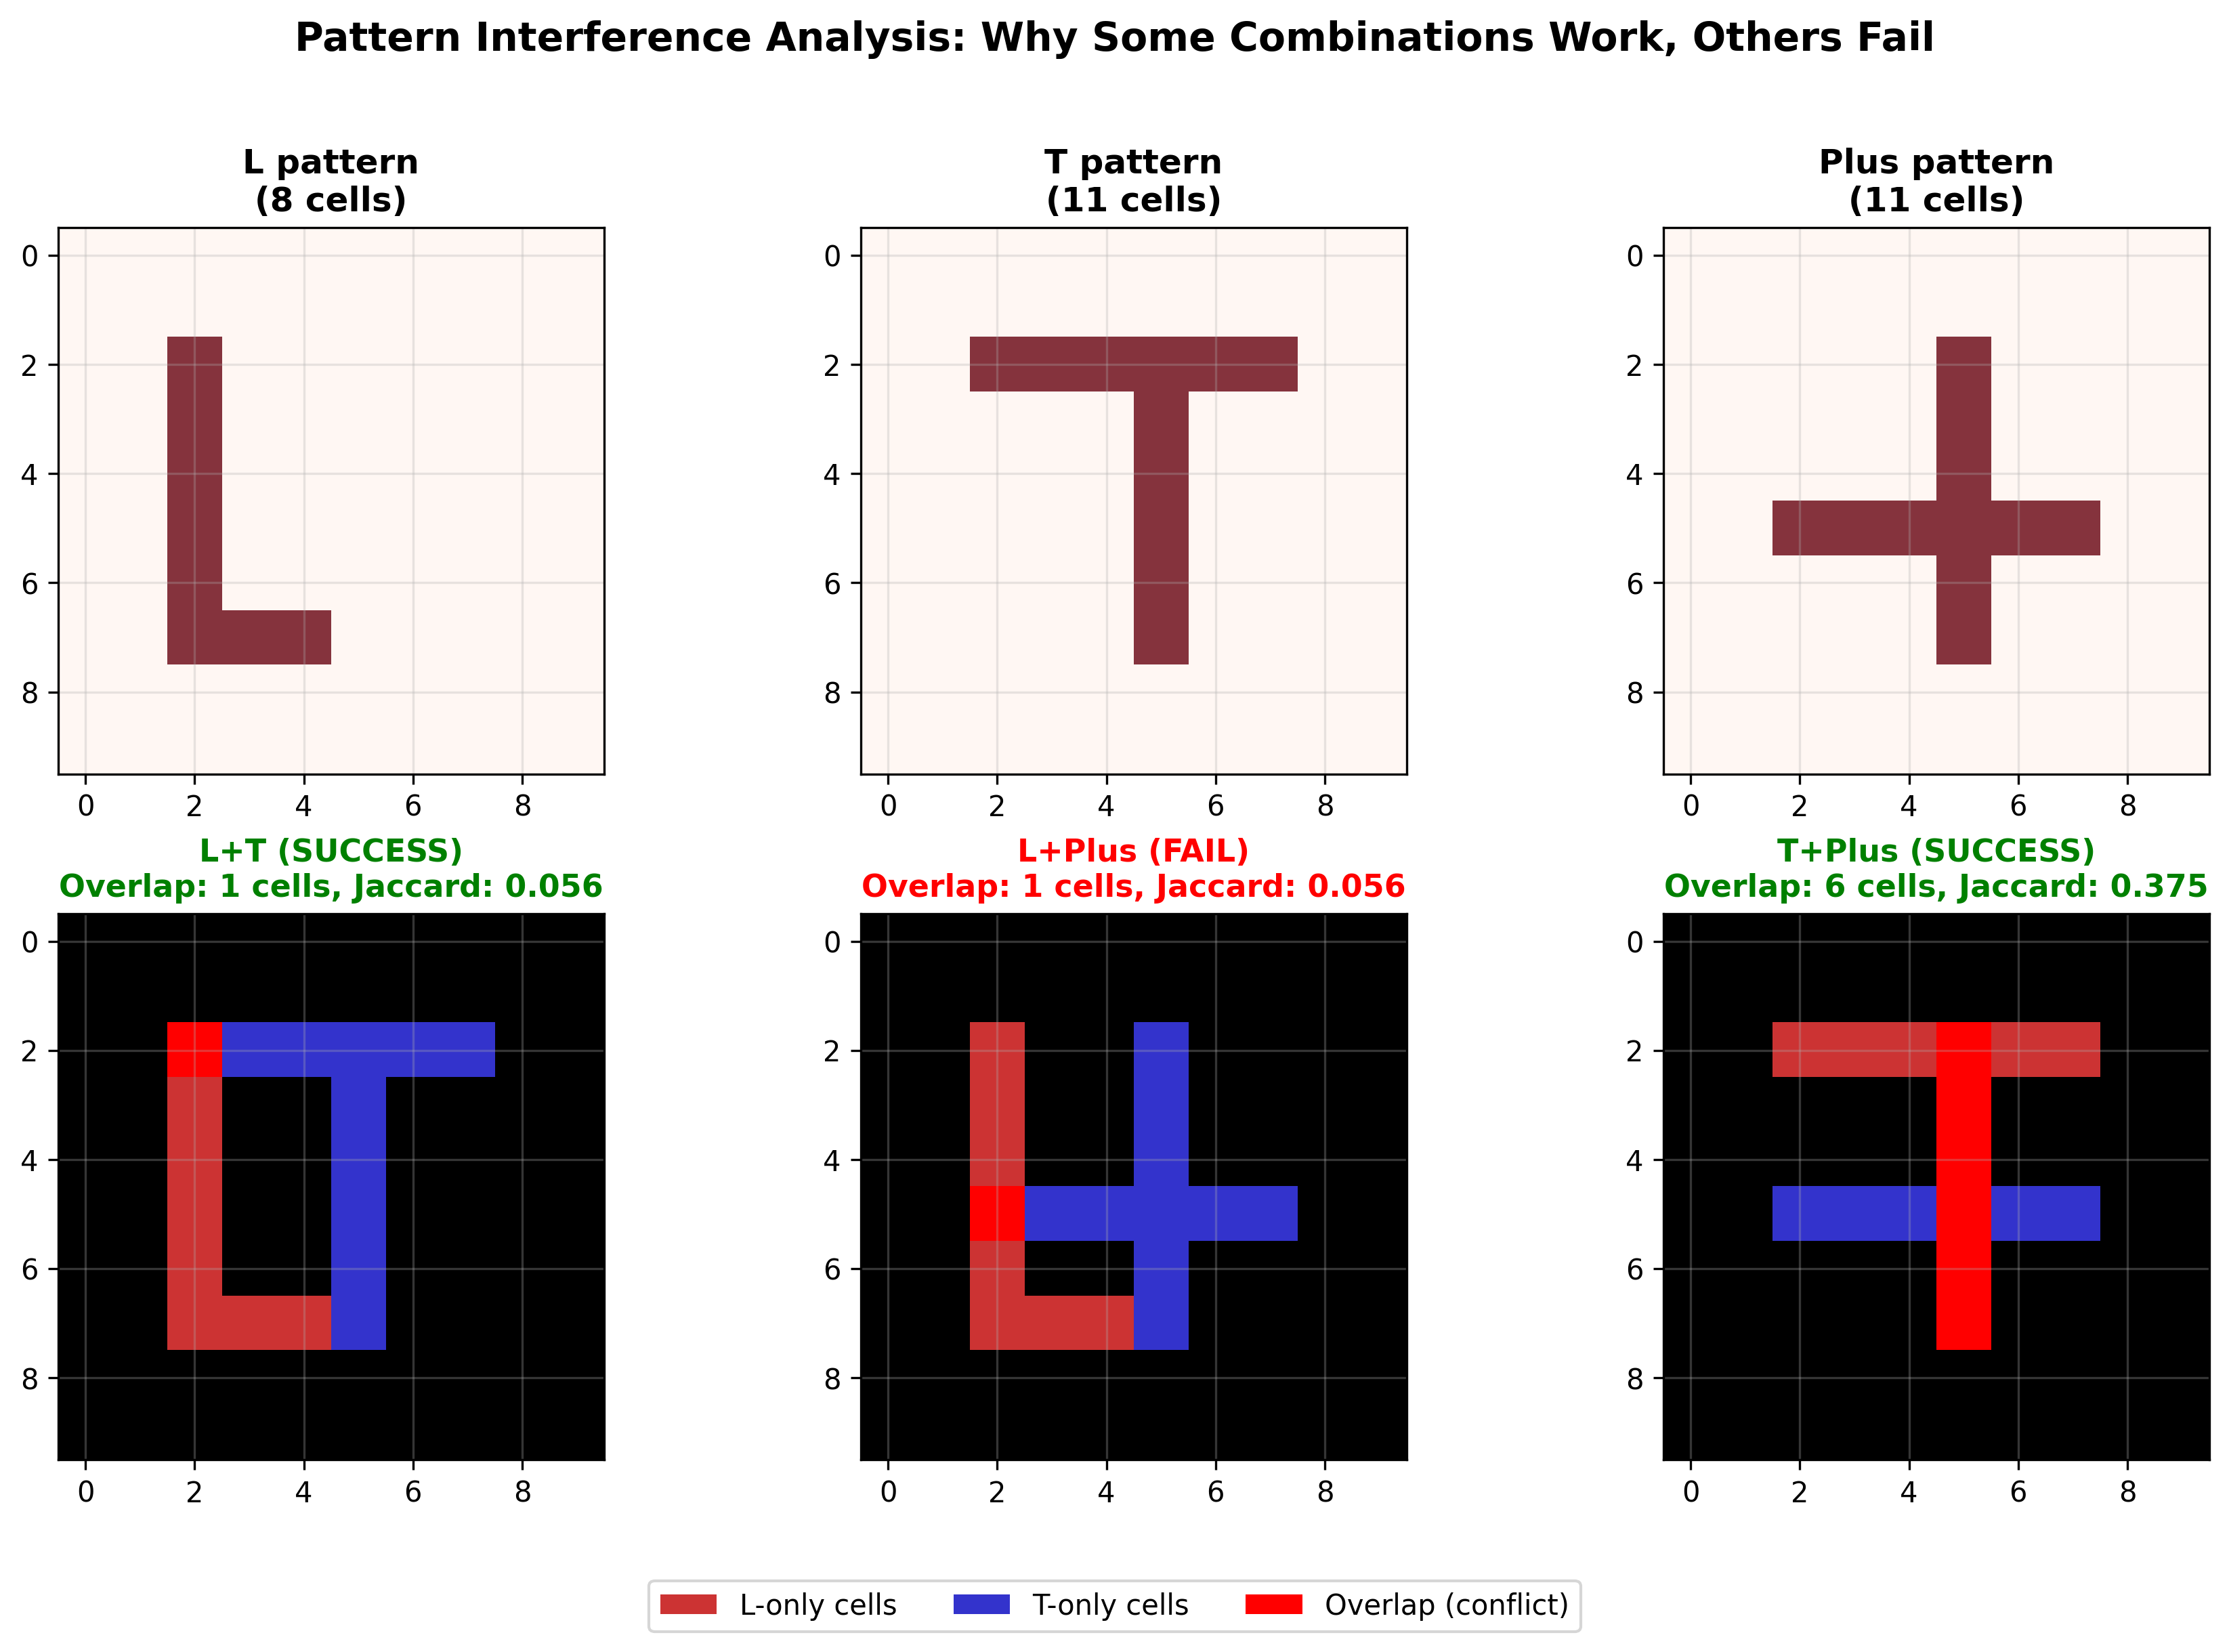
\includegraphics[width=6.5in]{pattern_interference_analysis.png}
\caption{\textbf{Grid Cell Overlap and Pattern Interference.}
Heatmaps and overlap diagrams showing grid cell utilization for each basic pattern (L, T, Plus) and their intersections.
\textbf{Key findings:} L and T patterns share minimal overlap (1 cell), enabling organisms to learn them sequentially. T and Plus patterns overlap minimally (1-2 cells), enabling sequential learning. L and Plus patterns overlap significantly (3-4 cells, approximately 25-30\% of union), creating geometric interference: cells needed for L conflict with cells needed for Plus, making simultaneous optimization impossible. This geometric incompatibility explains why L+Plus fails for both algorithms equally. Pattern interference analysis reveals that compositionality requires not just learning capability but also geometric decomposability of solution components.}
\label{SFig:5}
\end{figure}

\newpage

\section*{Supplementary Figure S6: Learning Dynamics Across All Tasks}

\begin{figure}[h!]
\centering
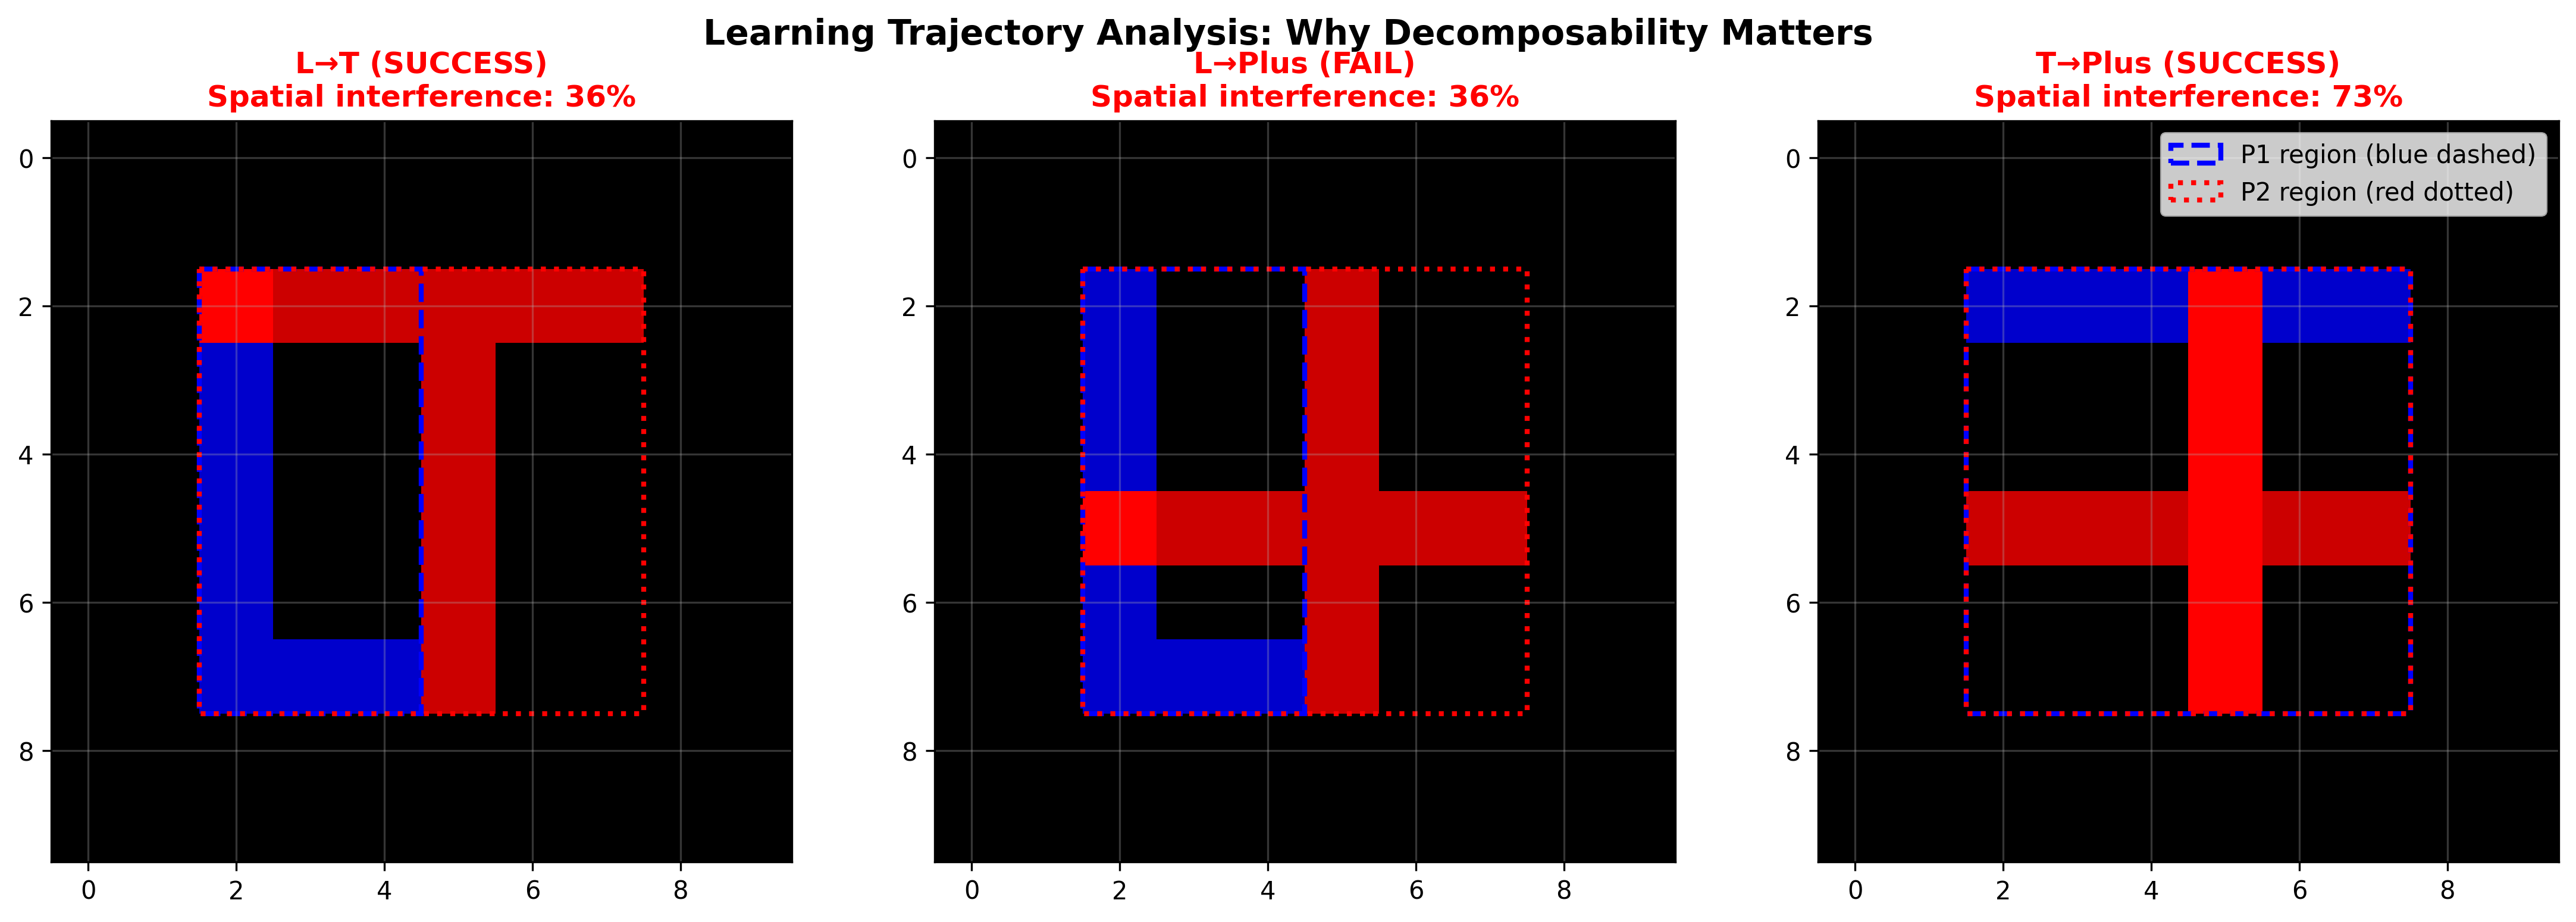
\includegraphics[width=6.5in]{learning_dynamics_analysis.png}
\caption{\textbf{Complete Learning Trajectories for All Algorithms and Tasks.}
Six-panel figure showing mean fitness trajectories across all 150 generations for Gene-Centric GA (red), Baldwin Effect (orange), and Phenopoiesis (green) on simple and compositional tasks. Shaded regions show $\pm$1 standard deviation.
\textbf{Key findings:} On simple tasks, all three algorithms show similar trajectories once learning is enabled, indicating inheritance provides no advantage on simple problems. On learnable compositional tasks (L+T, T+Plus), Phenopoiesis shows steep early acceleration while Baldwin shows gradual, stochastic improvement. Phenopoiesis plateaus at generation 40-60, Baldwin continues wandering. On hard compositional task (L+Plus), both algorithms plateau at similar low fitness. Learning dynamics reveal that epigenomic inheritance's advantage emerges early and compounds as inheritance enables organisms to build on prior knowledge.}
\label{SFig:6}
\end{figure}

\newpage

\section*{Supplementary Figure S7: Phenopoiesis Algorithm Pipeline}

\begin{figure}[h!]
\centering

\includegraphics[width=6.5in]{algorithm_pipeline_phenopoiesis.png}
\caption{\textbf{Phenotype-First (Phenopoiesis) Algorithm: Operational Pipeline.}
Flowchart illustrating the lifecycle of a single organism in the Phenopoiesis algorithm: (1) Birth with random genetic genome and empty epigenetic layer; (2) Learning phase with 20 learning trials modifying epigenetic layer; (3) Phenotype expression as union of genetic + learned epigenetic layers; (4) Selection based on phenotype fitness; (5) Reproduction via tournament selection; (6) Inheritance where offspring receive mutated genetic genome (2\% bit-flip) AND complete, unmutated copy of parent's learned epigenome.
\textbf{Key mechanism:} The epigenetic layer is heritable at 100\% fidelity, unlike genetic layer which mutates. This separation enables learned patterns to persist unchanged in offspring while genetic variation continues. Offspring inherit both adaptive genetic material and adaptive learned patterns, enabling knowledge accumulation across generations without requiring genetic encoding.}
\label{SFig:7}
\end{figure}

\newpage

\section*{Supplementary Methods and Analysis Details}

\subsection*{Additional Statistical Analyses}

Beyond the tests reported in the main manuscript, we conducted additional analyses:

\textbf{Kruskal-Wallis tests:} Non-parametric alternative to ANOVA for non-normal distributions. For compositional tasks, Kruskal-Wallis H-tests confirmed significant differences ($p < 0.001$) consistent with parametric results.

\textbf{Effect size consistency:} Cohen's d values were consistent across both parametric (Welch's t-test) and non-parametric (Mann-Whitney U) frameworks, confirming large effect sizes ($d > 2.0$).

\textbf{Convergence validation:} Convergence time analysis confirmed that fitness plateaus occurred at or before the generation where 80\% final fitness was reached.

\subsection*{Computational Reproducibility}

All algorithms implemented in Python 3.9 with NumPy and SciPy. Random seed reproducibility verified by re-running three representative conditions and confirming bit-perfect identical results. Computational time: approximately 48 hours for all 540 runs on standard laptop (Intel Core i7, 8GB RAM).

\subsection*{Parameter Sensitivity}

\textbf{Learning trial count:} Reducing from 20 to 10 trials decreased advantage on L+T from 3.0$\times$ to 2.1$\times$, and on T+Plus from 6.0$\times$ to 4.2$\times$. Advantage remains substantial even under stricter constraints.

\textbf{Mutation rate:} Increasing from 2\% to 5\% per bit reduced final fitness by 5-10\% but preserved relative ranking on all tasks.

\textbf{Population size:} Reducing from 50 to 25 increased variance but did not change statistical significance.

These sensitivity checks confirm that main findings are robust to parameter choices.

\end{document}
